% Gemini theme
% https://github.com/anishathalye/gemini
%
% We try to keep this Overleaf template in sync with the canonical source on
% GitHub, but it's recommended that you obtain the template directly from
% GitHub to ensure that you are using the latest version.

\documentclass[final]{beamer}

% ====================
% Packages
% ====================

\usepackage[T1]{fontenc}
\usepackage{lmodern}
\usepackage[size=custom,width=42in,height=42in,scale=1.3]{beamerposter}
\setlength{\paperwidth}{42in}
\setlength{\paperheight}{42in}
\usetheme{gemini}
\usecolortheme{gemini}
\usepackage{graphicx}
\usepackage{booktabs}
\usepackage{tikz}
\usepackage{pgfplots}
\usepackage{amsmath}
\usepackage{amssymb}
\usepackage[export]{adjustbox}
% ====================
% Lengths
% ====================

% If you have N columns, choose \sepwidth and \colwidth such that
% (N+1)*\sepwidth + N*\colwidth = \paperwidth
\newlength{\sepwidth}
\newlength{\colwidth}
\setlength{\sepwidth}{0.025\paperwidth}
\setlength{\colwidth}{0.3\paperwidth}

\newcommand{\separatorcolumn}{\begin{column}{\sepwidth}\end{column}}

\usepackage{subfig}
\usepackage{amsthm}
\usepackage{mathrsfs}
\usepackage{hyperref}
\usepackage{hyperref}
\usepackage{enumerate} 
% colors for easier looking for equations we refer to
% can be changed back to black in the future
% \usepackage[dvipsnames]{xcolor}
\hypersetup{
    colorlinks,
    citecolor=Amber,
    filecolor=blue,
    linkcolor=violet,
    urlcolor=Aquamarine
}
\usepackage{color}
\usepackage{mathtools}
\usepackage{float}
%%%%%%%%%%%%%%%%%%%%%%%%%%%%%%%%%%%%%%%%%%%%%%%%%%%%%%%%%%%%%%
%Here are some user-defined notations
\newcommand{\mres}{\mathbin{\vrule height 1.6ex depth 0pt width
		0.13ex\vrule height 0.13ex depth 0pt width 1.3ex}}
\newcommand{\RR}{\mathbf R}
\newcommand{\CC}{\mathbf C}
\newcommand{\ZZ}{\mathbf Z}
\newcommand{\ZZn}[1]{\ZZ/{#1}\ZZ}
\newcommand{\QQ}{\mathbf Q}
\newcommand{\rr}{\mathbb R}
\newcommand{\nn}{\mathbb N}
\newcommand{\cc}{\mathbb C}
\newcommand{\zz}{\mathbb Z}
\newcommand{\zzn}[1]{\zz/{#1}\zz}
\newcommand{\qq}{\mathbb Q}
\newcommand{\calB}{\mathcal B}
\newcommand{\calC}{\mathscr C}
\newcommand{\calM}{\mathcal M}
\newcommand{\calH}{\mathcal H}
\newcommand{\calG}{\mathcal G}
\newcommand{\calT}{\mathcal T}
\newcommand{\scrpT}{\mathscr T}
\newcommand{\E}{\textrm{Edge}}
\newcommand{\dist}{\operatorname{dist}}
\newcommand{\diam}{\operatorname{diam}}
\newcommand{\rad}{\operatorname{radius}}
\newcommand{\side}{\operatorname{side}}
\newcommand{\centerof}{\operatorname{center}}
% \newcommand{\bridge}{\operatorname{Bridge}}
% \newcommand{\edge}{\operatorname{Edge}}
% \newcommand{\CF}{\textrm{Cores}_{\textrm{Flat}}}
%\newcommand{\phantom}{\operatorname{Phantom}}
% \newcommand{\cores}{\operatorname{Cores}}
\newcommand{\latex}{\LaTeX}
\newcommand{\tex}{\TeX}
\newcommand{\sm}{\setminus} 
\newcommand{\dm}{(\mu)} 
\newcommand{\urlwofont}[1]{\urlstyle{same}\url{#1}}
%%%%%%%%%%%%%%%%%%%%%%%%%%%%%%%%%%%%%%%%%%%%%%%%%%%%%%%%%%%%%%
% \newtheorem{definition}{Definition}
\newtheorem{proposition}{Proposition}
\newtheorem{remark}{Remark}
% \newtheorem{lemma}{Lemma}
% \newtheorem{corollary}{Corollary}
% \newtheorem{theorem}{Theorem}
\newtheorem{innercustomthm}{Theorem}
\newenvironment{customthm}[1]
{\renewcommand\theinnercustomthm{#1}\innercustomthm}
{\endinnercustomthm}
\newtheorem{innercustomlemma}{Lemma}
\newenvironment{customlemma}[1]
{\renewcommand\theinnercustomlemma{#1}\innercustomlemma}
{\endinnercustomlemma}
\newtheorem{innercustomcorollary}{Corollary}
\newenvironment{customcor}[1]
{\renewcommand\theinnercustomcorollary{#1}\innercustomcorollary}
{\endinnercustomcorollary}

\title{Characterization of Rectifiable Measures that are Carried by Lipschitz Graphs}

\author{Charles Zhang, Yutong Wu}

\institute[shortinst]{Mathematics, Statistics, and Computer Science Department, Macalester College}

\logo{
\includegraphics[width=.12\textwidth]{images/maclogo.png}}
% ====================
% Body
% ====================
\usepackage{pgfplots}
\pgfplotsset{compat=1.7}

\begin{document}

\begin{frame}[t]
\begin{columns}[t]
\separatorcolumn

\begin{column}{\colwidth}

  \begin{block}{Background}

  From the analysis perspective,measures are used to define notions of size for sets. For example, traditionally the "size" of a curve is its arc length and the size of a square is its area. To understand how measures assign weight, we explore how they interact with various classes of sets. Here we can explore and find the characterization of measures which are carried by the Lipschitz graphs. Analysts are attracted by the property of Lipschitz graphs that we can find tangents almost everywhere on them.

  \end{block}

  \begin{block}{Definitions}
    To deep dive into the world of measures, we firstly need to introduce following definitions:\\
    \begin{itemize}
      \item \textbf{Measure} A \textit{measures} $\mu:\mathcal{M}\rightarrow\mathbb{R}$ is a function that assigns a "size" to sets in $\mathcal{M}$ according to the following rules:
	\begin{itemize}
		\item $\mu(E)\ge 0$ for all $E\in\mathcal{M}$ 
		\item $\mu(\emptyset)=0$.
		\item $\mu\left(\bigcup_{i=1}^\infty E_i\right)=\sum_{i=1}^\infty \mu(E_i)$ for a pairwise disjoint collection of set $\{E_i\}$
	\end{itemize}
	
	    \item  \textbf{Doubling Measure} We say that a measure $\mu$ is a K-doubling measure for some constant K if for all $r>0$ and $\mu$-a.e. $x$, 
   \begin{equation*}
       \mu(B(x, 2r))\leq K\mu(B(x,r))
   \end{equation*}
   
      \item \textbf{Dyadic Cubes} are squares on $\rr^2$ formed as cross product of half open intervals with side length as multiples of $1/2$.
    %   Fixed cubes formed by grid lines with its side length equals to multiples of $1/2$.
      \item \textbf{Point Cones} The bad cones on $\rr^2$ with respect to a line $V$ through the origin and $\alpha\in(0,1)$ are defined as
      \begin{equation*}
        \begin{split}
          C_\calB(x, V, \alpha) &:= \{y\in \rr^n: \dist(y-x, V) > \alpha |x-y|\} 
    \end{split}
      \end{equation*}
      Visualization of point cones and several numerical relationship is illustrated in Figure {\color{violet}(b)} below.
      \item \textbf{Cube Cones} Bad Cube cones used in our work are defined as $C^{I}_{\calB}(Q, V, \alpha) &:= \bigcap_{x\in Q} C_\calB(x, V, \alpha)$, and discretely defined as
      \begin{equation*}
        \begin{split}
            C_\calB^{I,1}(Q, V, \alpha) &:= \{R: R\cap C_\calB^I(Q, V, \alpha) \neq \emptyset\} \\
            C_\calB^{I,2}(Q, V, \alpha) &:= \{R: R\subset C_\calB^I(Q, V, \alpha)\}
          \end{split}
      \end{equation*}
      where $R$ is the dyadic cube same as $Q$.
    %   $C_\calB^1(Q, V, \alpha)$ and $C_\calB^2(Q, V, \alpha)$ are formed by the union and intersection of all point cones $C_\calB(x, V, \alpha)$ where $x\in Q$ respectively. 
    Visualization of three definitions of cube cones are shown in the shaded area in Figure {\color{violet}(b)} below.
      
    %   bad cube cones and the cones centered at the two ends of the diagonal of cubes formed by purple and orange lines are point bad cones. 
    \begin{figure}
      \centering
      \subfloat[\centering Point Cones ]{{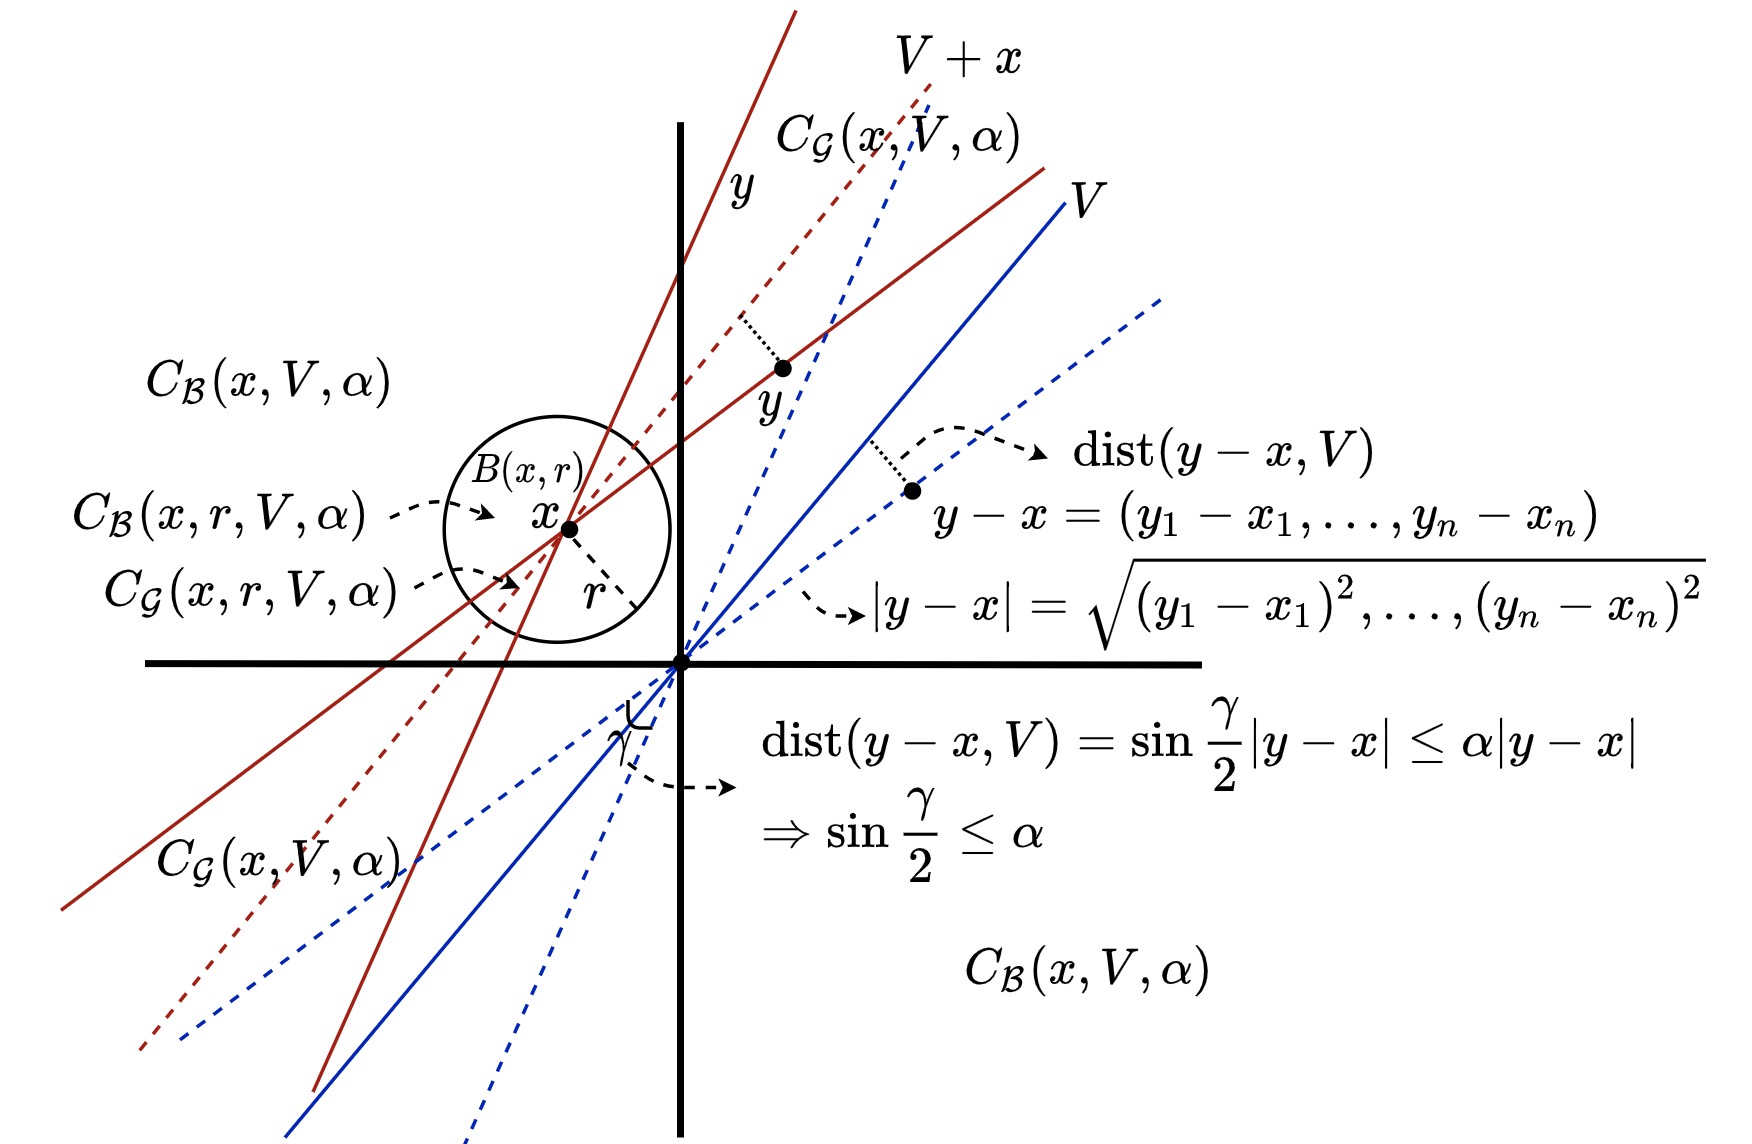
\includegraphics[width=0.5\textwidth]{images/conedef.png} }}%
    % \qquad
    \subfloat[\centering Cube Cones] {{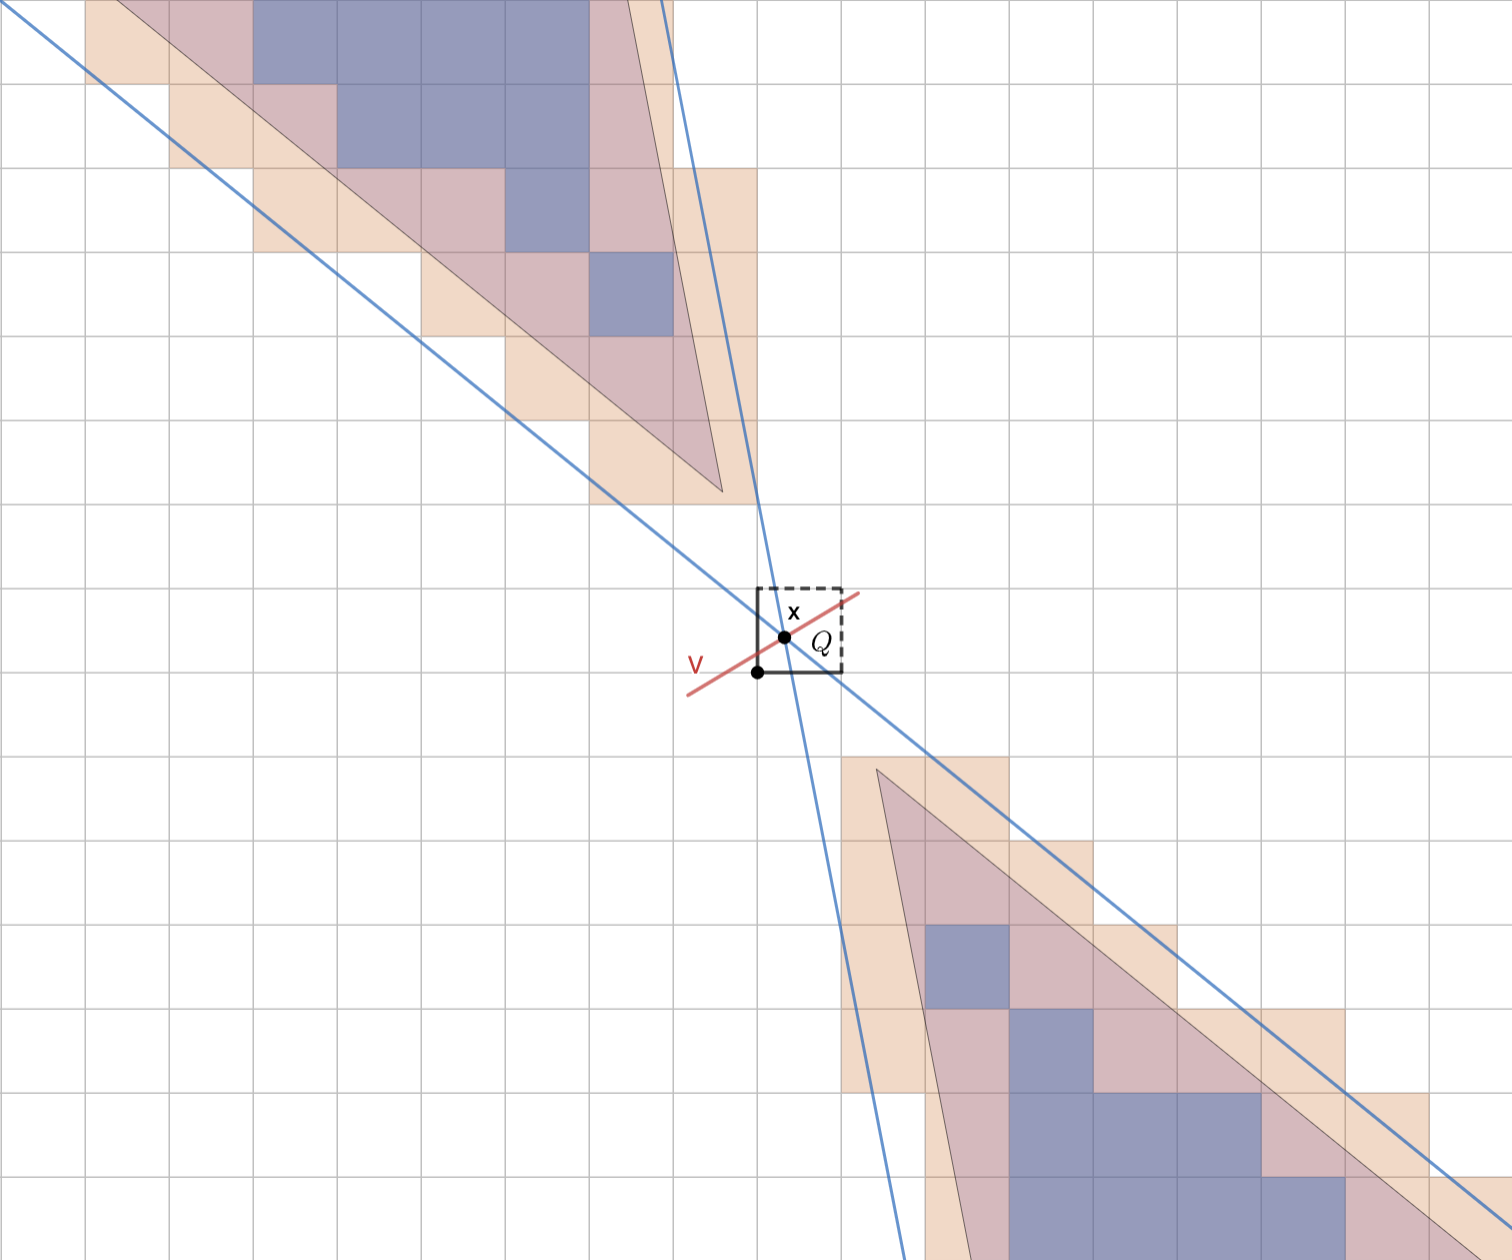
\includegraphics[width=0.5\textwidth]{images/cubecone.png} }}%
    \caption{Cones Visualization}%
    \label{fig:conevis}%
    %   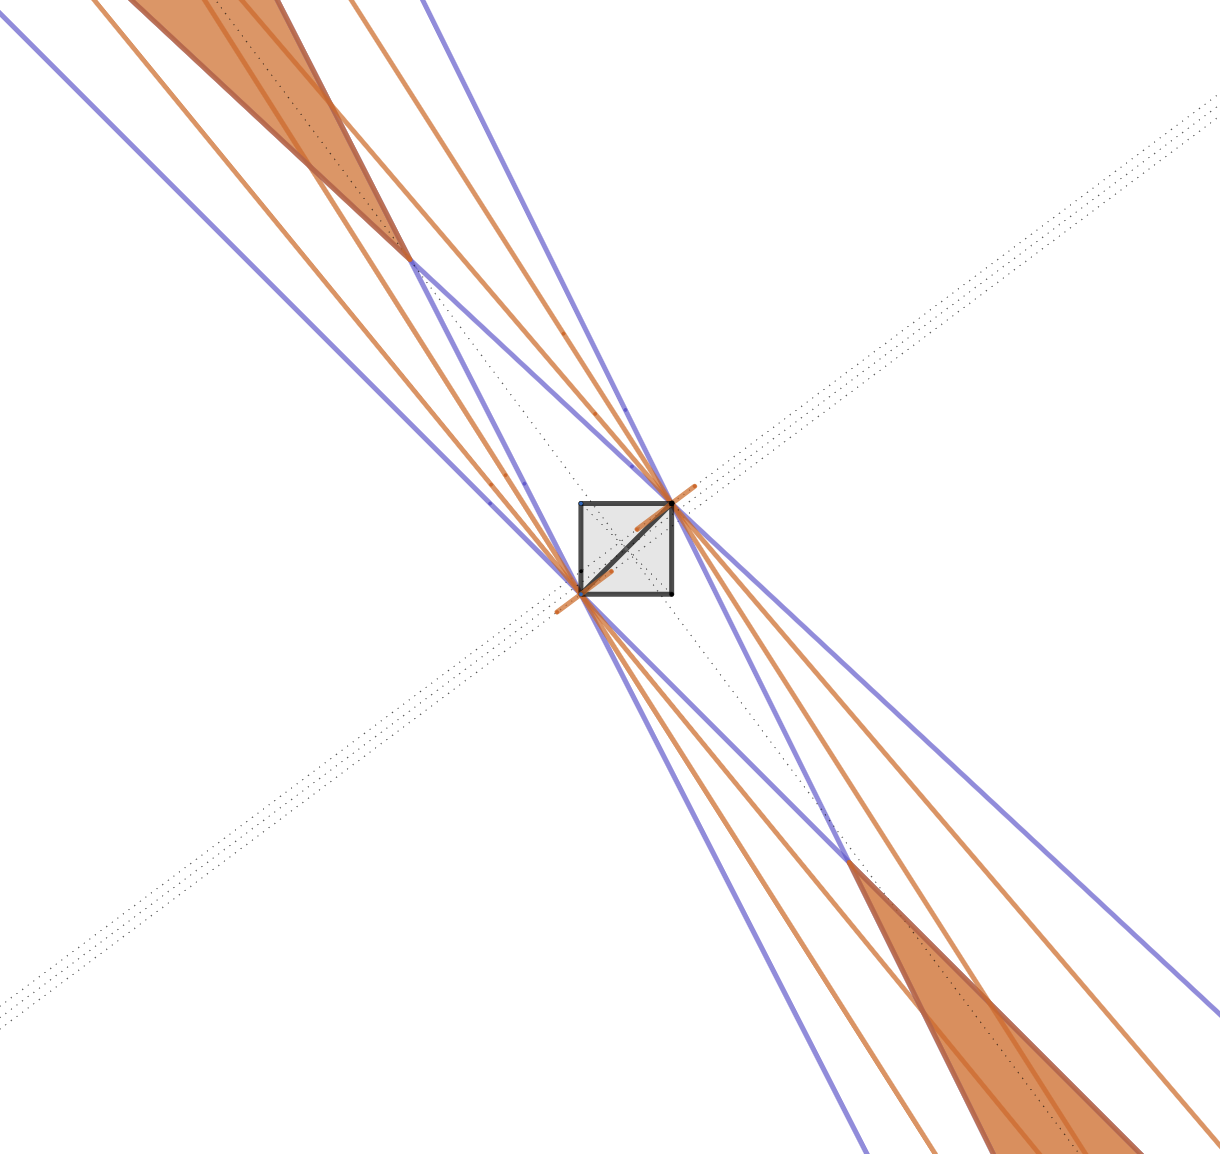
\includegraphics[]{images/cones.png}
    %   \caption{example of point and cube cones}
    \end{figure}
    % \item \textbf{Lipschitz Graph}
    % Suppose $g(x)$ is a Lipschitz function, then we have $G(x) = (x, g(x))$ satisfies:
    % $$
    % |x - y| \leq |G(x) - G(y)| \leq \sqrt{1+c^2}|x - y|
    % $$
    % for $0<c<\infty$ and we call $G(x)$ the graph function of Lipschitz function $G(x)$
        \item \textbf{Lipschitz Function} The function $f$ is called Lipschitz if
        $$
        |f(x)-f(y)| \leq c|x-y| \quad(x, y \in \rr, 0<c<\infty)
        $$
        \item \textbf{Lipschitz Graph}
        Let $f: V\rightarrow V^\bot$ be a Lipschitz function. Then $\operatorname{Graph}(f) = \{(x, f(x)): x\in V\}$ is a Lipschitz graph
        
        \item \textbf{Carried}   Let $(\mathbb{R}^2, \mathcal{M})$ be a measurable space, and let $\mathcal{N} \subset \mathcal{M}$ be a family of measurable sets. We say $\mu$ is carried by $\mathcal{N}$ if there exist countably many $N_{i} \in \mathcal{N}$ such that $\mu\left(\mathbb{R}^2 \backslash \bigcup_{i} N_{i}\right)=0$
    \end{itemize}
    When we say $\mu$ is carried by Lipschitz graphs, it is equivalent that there exists a subset of $\rr^n$ is contained $\mu$-a.e. in countably many Lipschitz graph. 
\end{block}

\end{column}

\separatorcolumn

\begin{column}{\colwidth}
    % \heading{Rademacher's Theorem}
    % If $U$ is an open subset of $\rr^n$ and $f: U \rightarrow \rr^m$ is a Lipschitz function, then f is differentiable almost everywhere in $U$; that is, the points in $U$ at which $f$ is not differentiable form a set of Lebesgue  measure zero.
\begin{block}{Related Work}

\heading{Geometric Lemma\cite[Lemma 4.7]{de2008rectifiable}}
    Let $F \subset \rr^2$, $V$ be a line through the origin, and $\alpha \in(0,1)$. If
$$
F \cap C_{\mathcal{B}}(x, V, \alpha)=\emptyset \text { for all } x \in F
$$
then $F\subset \Gamma$ where $\Gamma$ is a $1$-Lipschitz graph with respect to $V$ and the Lipschitz constant corresponding to $\Gamma$ is at most $1+1 /\left(1-\alpha^{2}\right)^{1 / 2} .$

    % Let $F \subset H$, let $V$ be an $m$-dimensional linear plane
    \begin{figure}
      \centering
      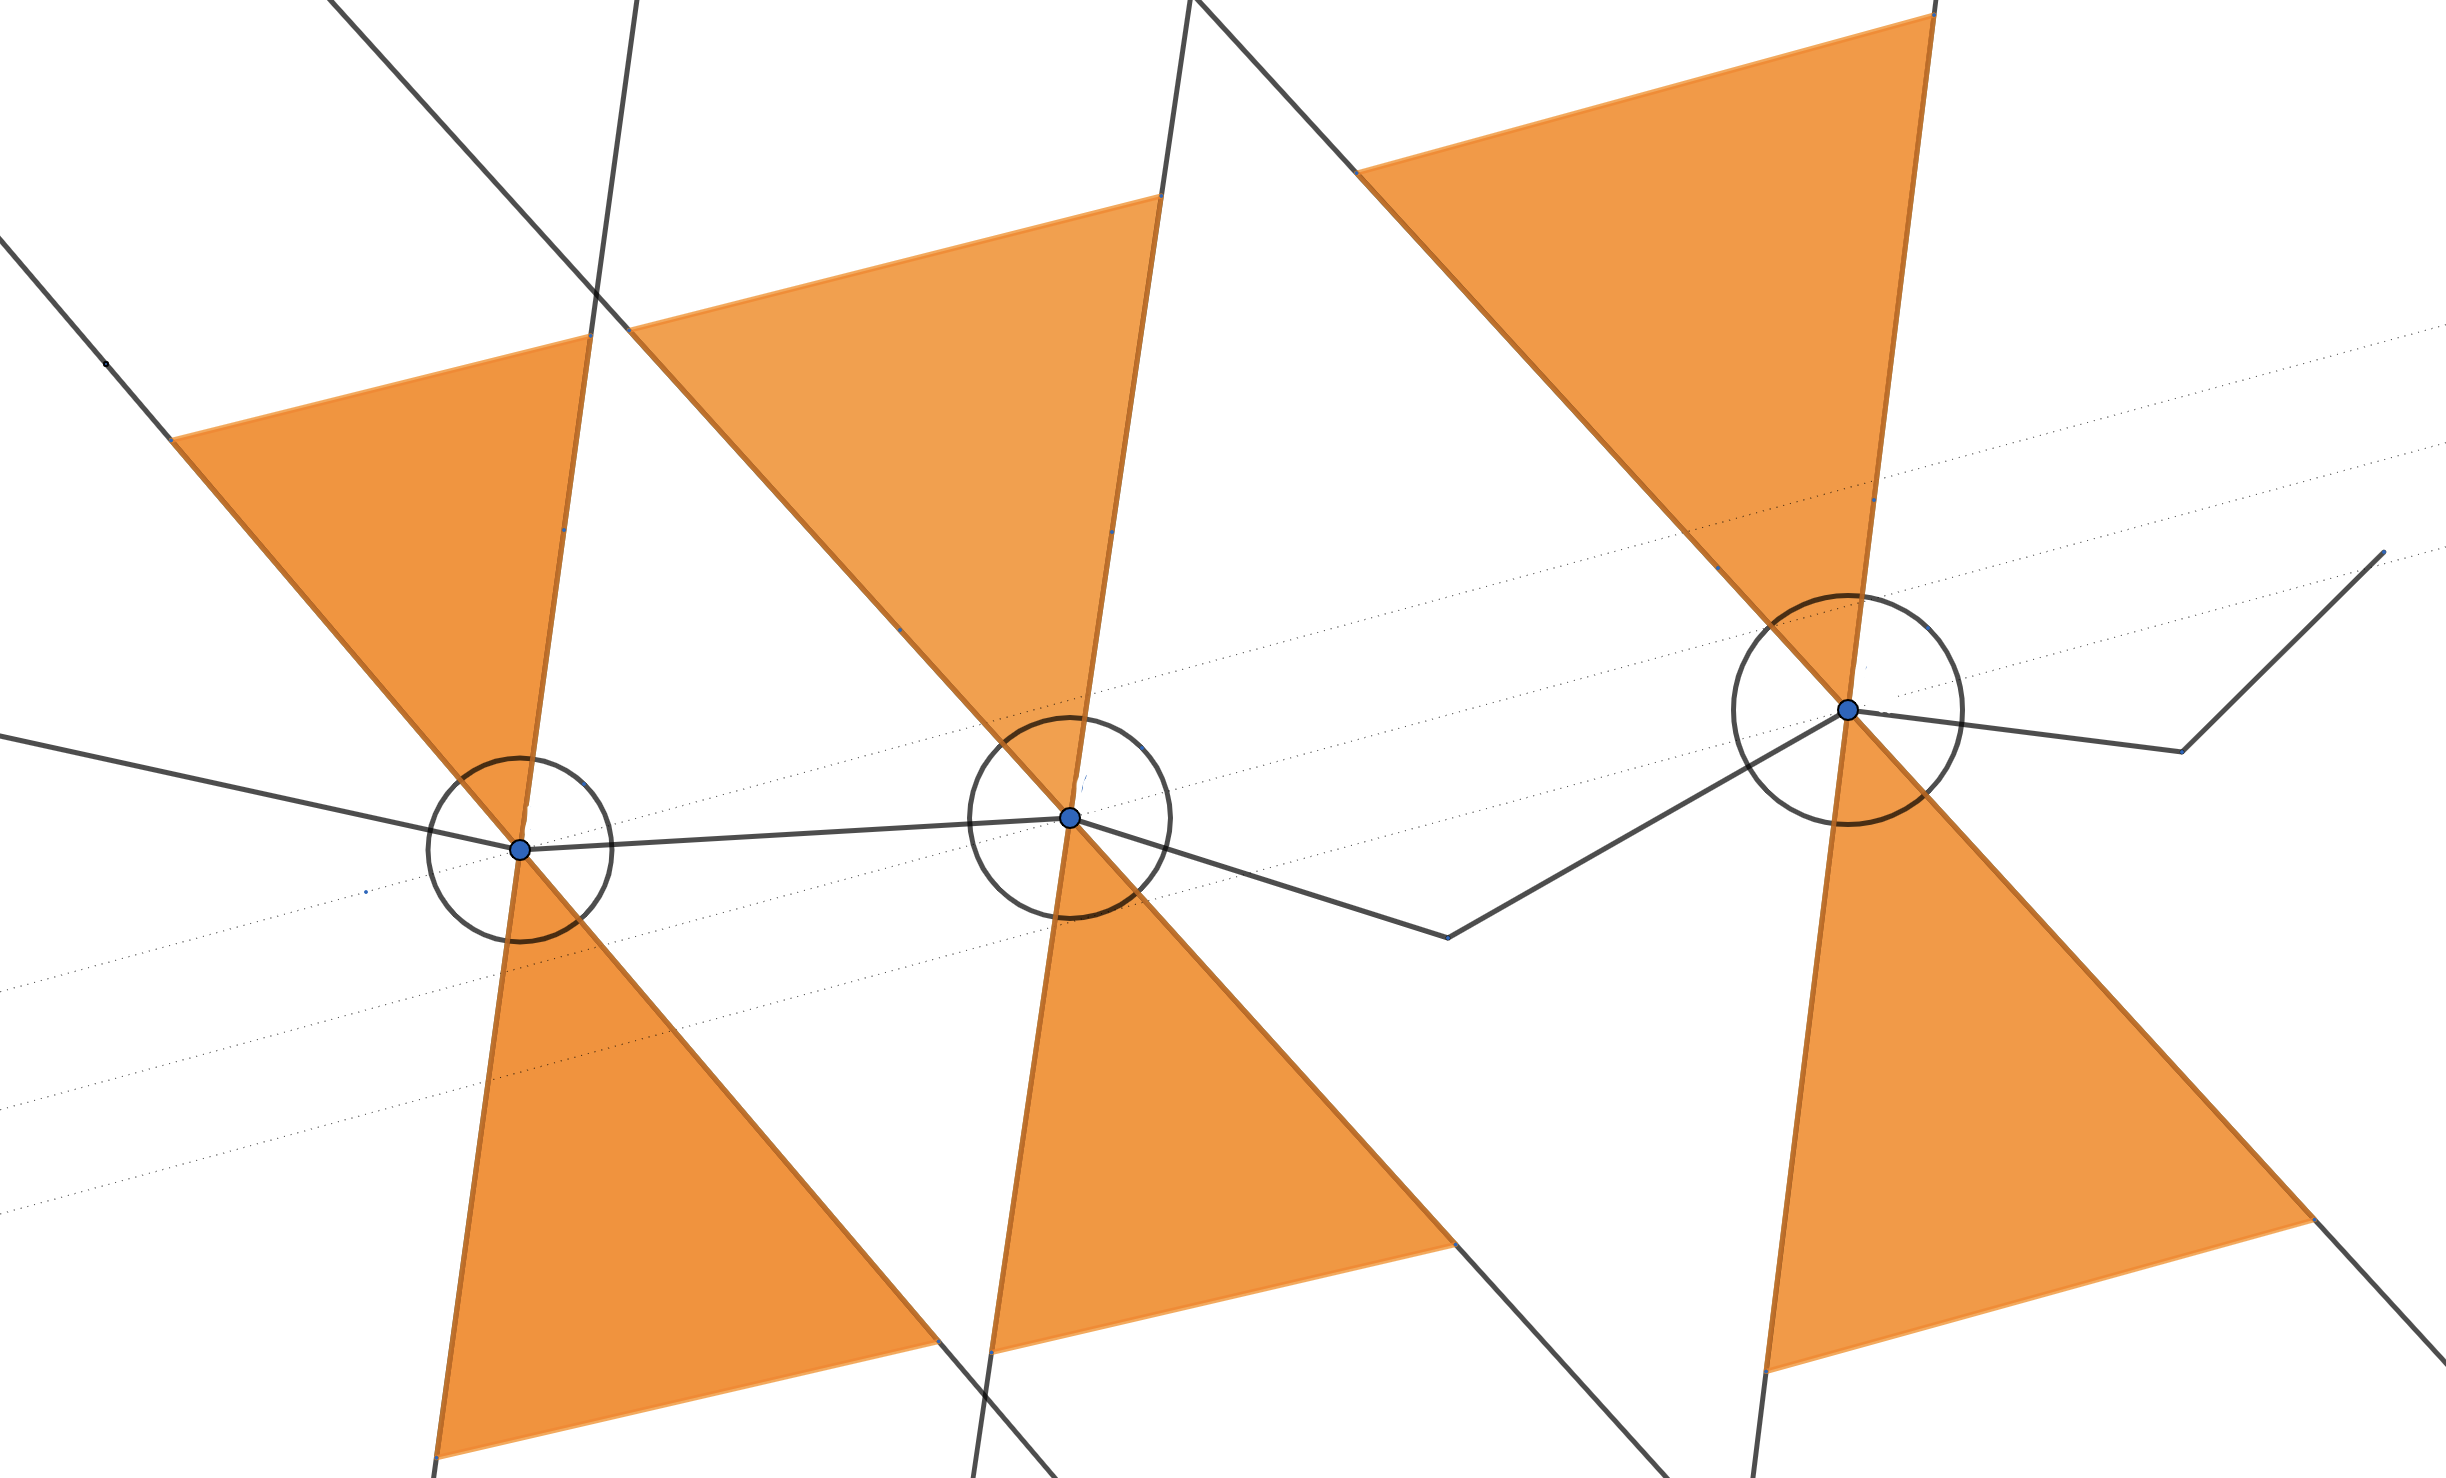
\includegraphics[width = 6.5in]{images/old method.png}
      \caption{An example of the geometric lemma}
    \end{figure}

    % \heading{Measure Differentiation \cite[Corollary 2.14]{mattila1999geometry}}\label{coro:mattila-coro-2.14}
    % If $A \subset \rr^{n}$ is $\mu$ measurable, for $\mu$ almost all $x \in \rr^{n} \backslash A$, the limit
    %     $$
    %     \lim _{r \downarrow 0} \frac{\mu(A \cap B(x, r))}{\mu(B(x, r))} = 0
    %     $$
    
%every single points there might be uncountably many points, but the dyadic cube can solve this problem.
  \end{block}

  \begin{block}{Main Result}
    \heading{Theorem A}\label{thmA}
    Let $\mu$ be a $K$-doubling measure on $\rr^2$. Then for $\mu$-a.e. $x\in\rr^2$ contained in the dyadic cube $Q$, there exists a line $V$, $\alpha\in(0,1)$, and $s = s(\alpha)\in\nn$ such that 
    \begin{itemize}
        \item (\textit{Sufficient Condition}) if the limit
        \begin{equation}\label{eq:limBC-2sQ-0}
            \lim_{Q\downarrow x}\frac{\mu(C_\calB^{I,1}(Q, V, \alpha)\cap 2sQ)}{\mu(2sQ)} = 0
        \end{equation}
        then $\mu$ is carried by Lipschitz graphs with respect to $V$ and the Lipschitz constant for each graph is at most $1+1/(1-\alpha^{\prime2})^{1/2}$ for any $\alpha < \alpha^\prime<1$.
        
        \item (\textit{Necessary Condition}) if $\mu$ is carried by Lipschitz graphs with respect to $V$ and the Lipschitz constant at most $\alpha/(1-\alpha^2)^{1/2}$, then (\ref{eq:limBC-2sQ-0}) holds.
    \end{itemize}
    
    
    \textit{Note}: $C_\calB^{I,1}$ in the limit can be replaced with $C_\calB^I$ as well.
    
  \end{block}
\begin{block}{Proved New Lemmas}

    To fully prove the sufficient and necessary condition of Theorem {\color{violet}A}, we first provide lemmas below.
    
    
    \heading{Lemma 1 (Choices of Scaling for Containment)}
        For $0<\alpha<\alpha^\prime<1$, a line $V$, a dyadic cube $Q$ in $\rr^2$, and $s\geq \frac{3\sqrt{2}(1+\alpha)}{\alpha^\prime-\alpha}$. Let $2R$ be a dilation of a cube $R$ such that $R$ is the dyadic cube with the same side length as $Q$ and
    \begin{equation*}
        \dist(Q, 2R)\geq s\cdot \side Q
    \end{equation*}
    then
    \begin{enumerate}[(i)]
        \item \label{lemma-1:s-guarantee-containQ-between-2alpha} if $2R\subset C_\calB^{I,1}(Q, V, \alpha^\prime)$, then $2R\subset  C_\calB^{I,2}(Q, V, \alpha)$.
        \item \label{lemma-2:s-guarantee-containQ-between-2alpha} if for $n = n(s) \in \nn$ such that $2^n\geq 2(\sqrt{2}+1)s + 3\sqrt{2}$, then $2sQ\subset 2^n R $.
        \item \label{lemma-3:s-guarantee-containQ-between-2alpha} if for $m = m(s) \in \nn$ such that $2^m \geq (3\sqrt{2}+2)s + 3\sqrt{2}$, then $3sQ\subset 2^m R$. 
    \end{enumerate}
    
    \heading{Lemma 2 (Doubling Property for Cubes)}
    Suppose that a doubling measure $\mu$ on $\rr^2$ is $K-$doubling, then for any dyadic cube $Q$ containing $\mu$-typical point $x$, 
    \begin{equation}\label{eq:doubling4cubes}
        \mu(2^n sQ)\leq K^{3n-3} \mu(2sQ)
    \end{equation}
    where $s, n\in \nn, n\geq 2$.
    \end{block}
\end{column}


\separatorcolumn

\begin{column}{\colwidth}


    \begin{block}{Main Steps of the Proof}
    \heading{Proof of \textit{Sufficient Condition}}
    Fix a $Q_k$ with a large enough $k$ and construct sets
    {\small{
    \begin{equation*}
        \begin{split}
            S_{Q_k} &:= \left\{2R_k: \dist(2R_k, Q_k)\geq \frac{1}{2}s\cdot\side Q_k, 2R_k\cap(2sQ_k\cap C_\calB^{I, 1} (Q_k, V, \alpha^\prime))\neq \emptyset\right\} \\
            S_{Q_k}^\prime &:= \left\{2R_k: \dist(2R_k, Q_k)\geq \frac{1}{2}s\cdot\side Q_k, 2R_k\subset 2sQ_k\cap C_\calB^{I, 1} (Q_k, V, \alpha^\prime)\right\} \\
            S_{Q_k}^{\prime\prime} &:= S_{Q_k} \setminus S_{Q_k}^\prime
        \end{split}
    \end{equation*}
    }}
    where $R_k$ is a dyadic cube with the same side length as $Q_k$ and $2R_k$ is its dilation. By Lemma {\color{violet}1}, Lemma {\color{violet}2}, (\ref{eq:limBC-2sQ-0}), and proof by contradiction we show $\mu(S_{Q_k}) = 0$. With some analysis, we show 
    \begin{equation*}
        \begin{split}
            \mu(C_\calB(x, r, V, \alpha^\prime))\leq \mu\left( \bigcup_{i=k}^\infty \left\{S_{Q_i}:x\in Q_i\subset Q_k \right)\}\right) = 0
        \end{split}
    \end{equation*}
  By the Geometric Lemma and \cite[Corollary 7.1]{naples2020rectifiability}, the sufficient condition holds immediately. 
    
    
    \begin{figure}
      \centering
      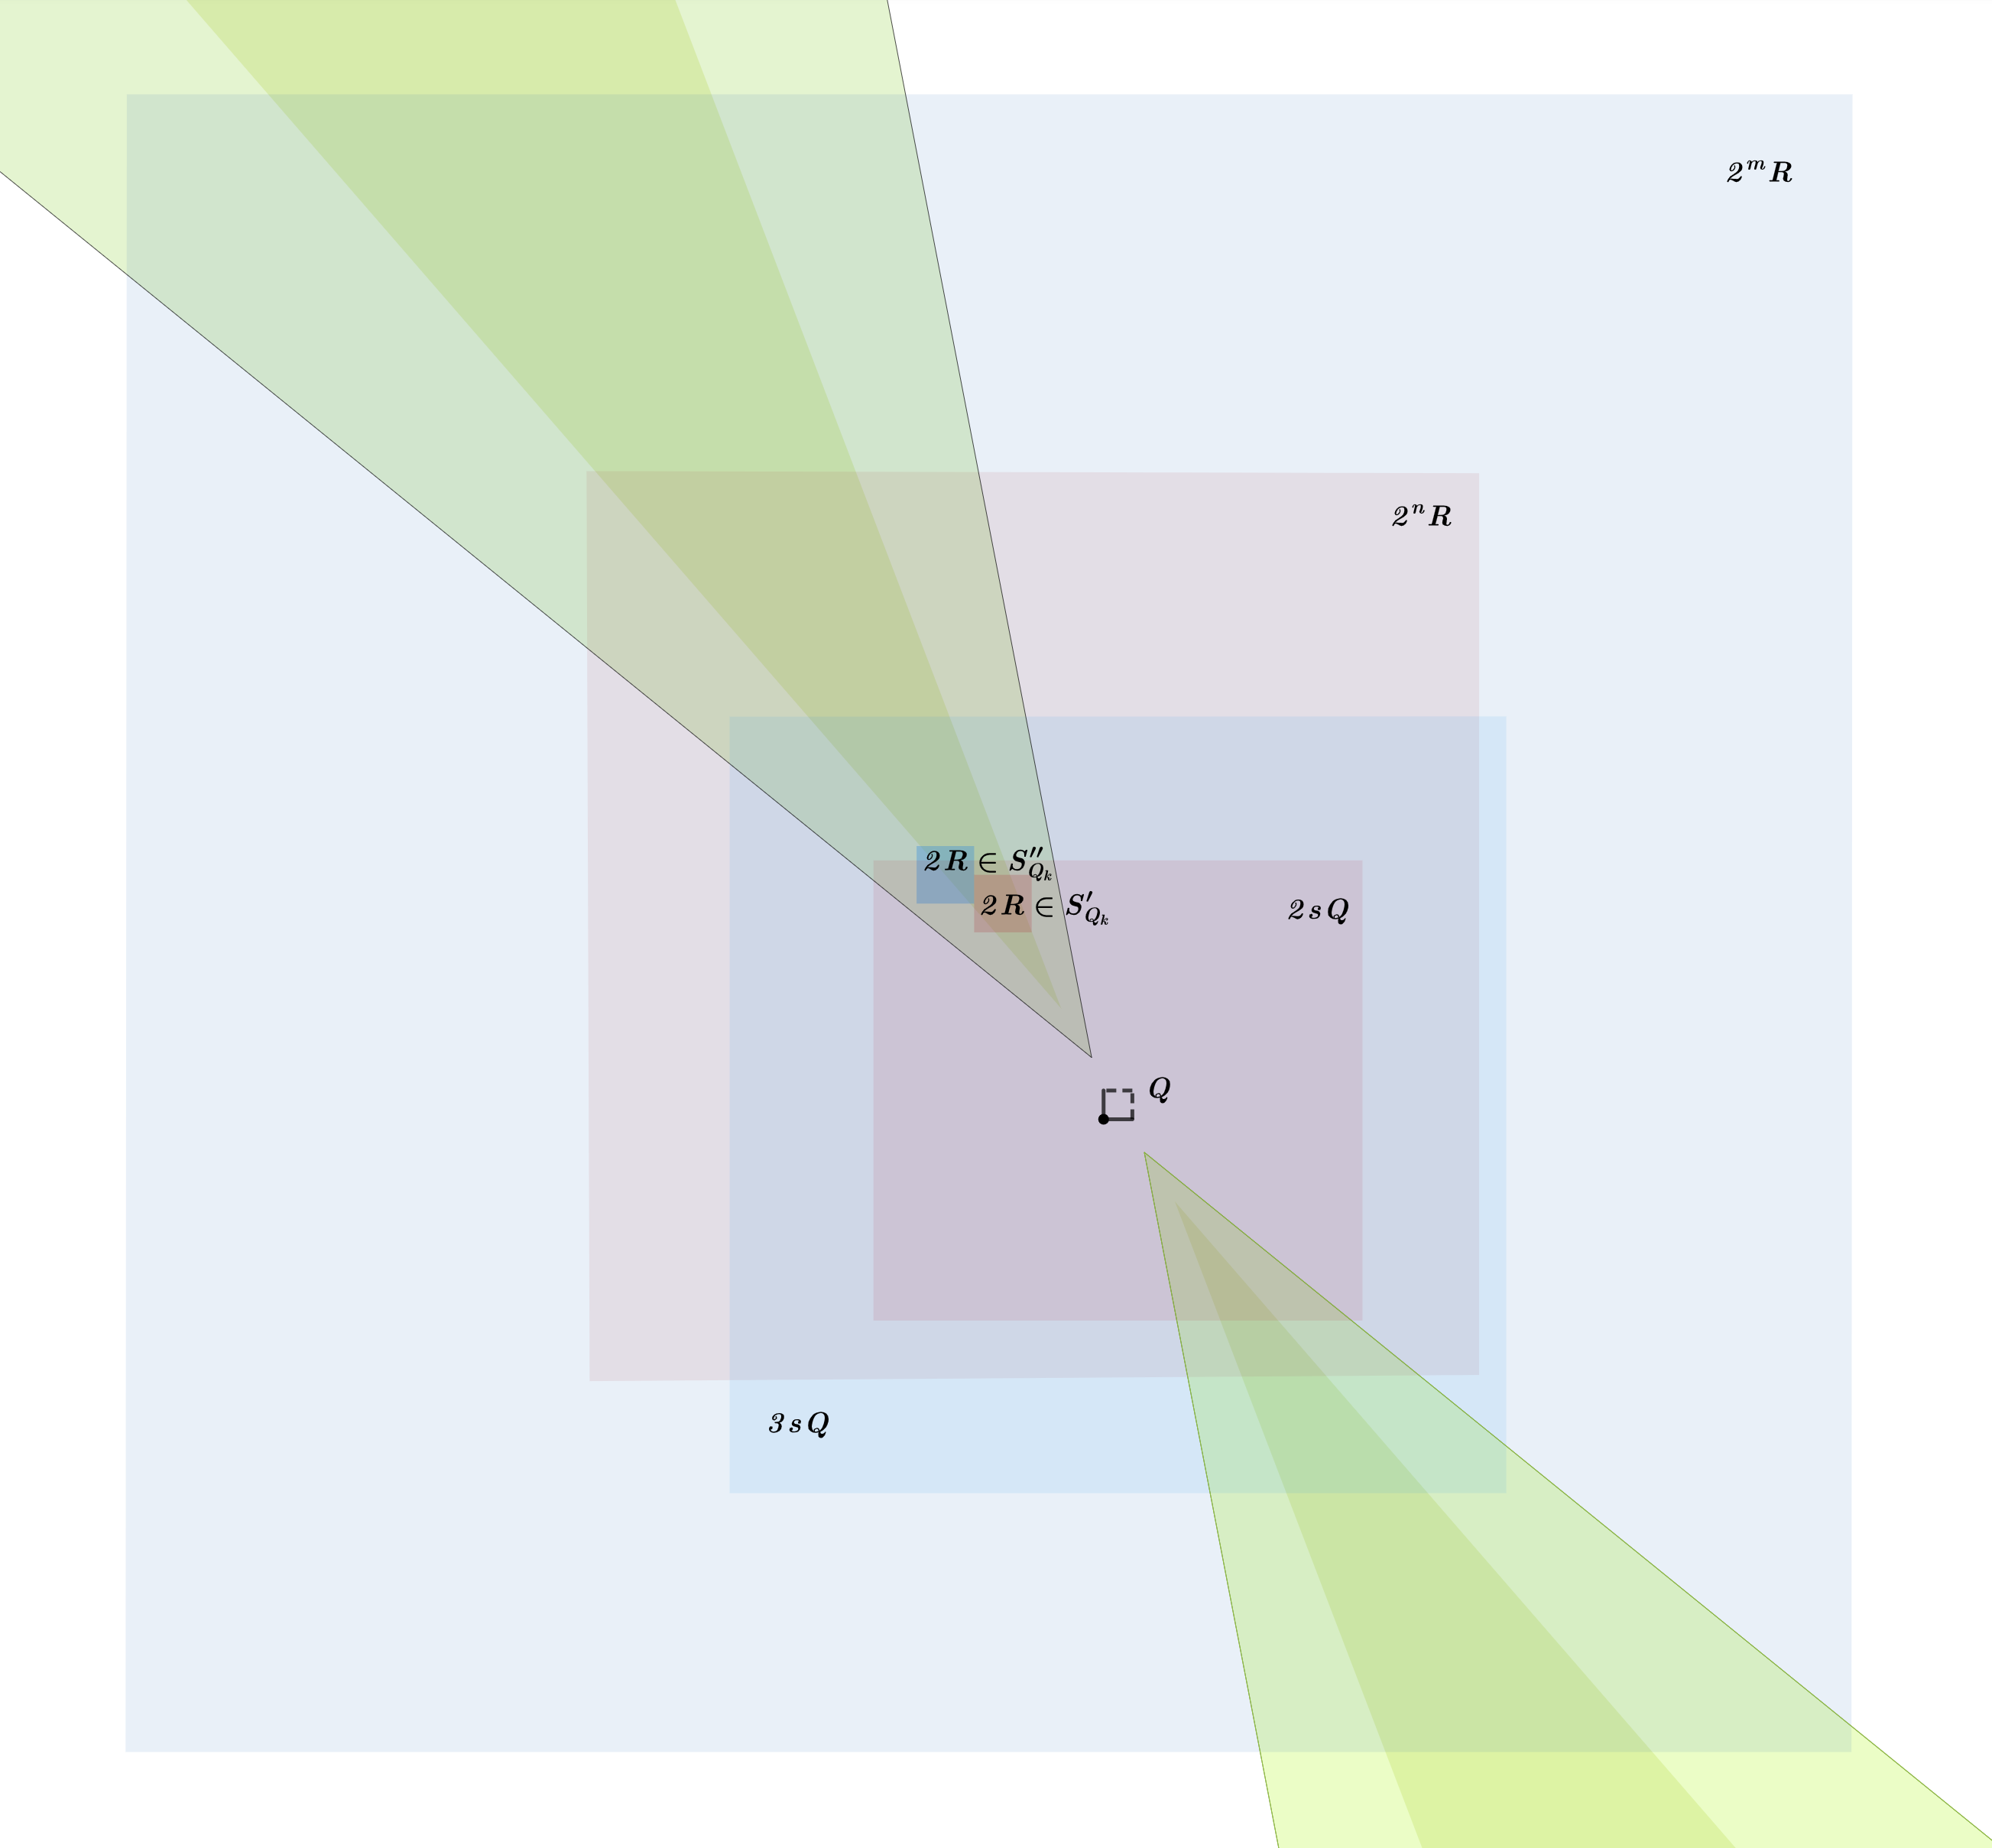
\includegraphics[width = 0.9\textwidth]{images/2sq.png}
      \caption{Visualization of the proof for Sufficient Condition}
    \end{figure}
        
    
    
    \heading{Proof of \textit{Necessary Condition}}
    By the assumption, we show
    \begin{equation}\label{containment-necessary-condition}
    \begin{split}
        C_\calB^{I,1}&(Q_k, V, \alpha) \cap 2sQ_k \subset C_\calB(x,V, \alpha) \cap 2sQ_k \\ & \subset 2sQ_k \setminus C_\calG(x, V, \alpha) \subset 2sQ_k \setminus E 
    \end{split}
    \end{equation}
    where $E$ consists of $\mu$-a.e. $x$. By Measure Differentiation \cite[Corollary 2.14]{mattila1999geometry} and Lemma {\color{violet}2} if we set $r_k = (\sqrt{2}s + \sqrt{2}/2) \cdot 2^{-k}$, we show
    {\small{
    \begin{equation}\label{temp}
        \begin{split}
            \lim_{k\rightarrow \infty} \frac{\mu(2sQ_k \setminus E)}{\mu(2sQ_k)} 
            \leq \lim_{k\rightarrow \infty} \frac{\mu(2sQ_k \setminus E)}{K^{-3}\mu(4sQ_k)} 
            \leq K^3 \lim_{k\rightarrow \infty} \frac{\mu(B(x, r_k) \setminus E)}{\mu(B(x, r_k))} = 
            0
        \end{split}
    \end{equation}
    }}
    Combining (\ref{containment-necessary-condition}) and (\ref{temp}),
    \begin{equation*}
        \lim_{k\rightarrow \infty}\frac{\mu(C_\calB^{I,1}(Q_k, V, \alpha)\cap 2sQ_k)}{\mu(2sQ_k)} =0
    \end{equation*}
    This completes the proof of the necessary condition. 
    \end{block}
    



  

  \begin{block}{References}

    \nocite{*}
    \footnotesize{\bibliographystyle{alpha}\bibliography{poster}}

  \end{block}


%  \begin{figure}
%     
\includegraphics[width=.46\textwidth, right]{images/maclogo.png}
% \end{figure}
\end{column}

\separatorcolumn


\end{columns}
\end{frame}

\end{document}
